\documentclass[11pt]{article}
\usepackage[margin=1in]{geometry}
\usepackage{amsmath,amssymb}
\usepackage{graphicx}
\usepackage{booktabs}
\usepackage{multirow}
\usepackage{xcolor}
\usepackage{hyperref}
\hypersetup{colorlinks=true,linkcolor=blue,citecolor=blue,urlcolor=blue}

% Marks a table cell / number that must be produced by an experimental run.
\newcommand{\TBD}{\textcolor{red}{\texttt{[run]}}}

\title{\textbf{Where Does a VLM Refuse?}\\
Modality-Entangled Safety Subspaces, Cross-Modal Abliteration,\\
and Retained Offensive-Cyber Capability}
\author{Akan Mukhametgali \\ MU}
\date{\today}

\begin{document}
\maketitle

\begin{abstract}
Abliteration---removing the low-dimensional ``refusal direction'' from an aligned
model's activation or weight space---has become a standard probe of how brittle
safety alignment is, and a family of defenses now hardens language models against
it. Almost all of this work, attacks and defenses alike, lives in the \emph{text}
representation. We ask a question specific to vision-language models (VLMs): is
there a refusal direction carried by the \emph{visual} pathway that is distinct
from the text refusal cone, and if so, does it make text-space defenses
circumventable through the image channel? We formalize refusal in a VLM as a
\emph{union of modality-conditioned cones}, a text cone $R_T$ and a visual cone
$R_V$, and treat activation abliteration and weight-space model souping as dual
operators on this union. We contribute (i) a layer-wise cross-modal refusal map
that measures the principal angles between $R_T$ and $R_V$ and the energy of
$R_V\setminus R_T$ that text edits miss, shown scale-robust across three VLMs; (ii) a
\emph{causal} probe that injects known safety onto a base VLM and isolates a
text$\rightarrow$image refusal-transfer gap; (iii) an honest-negative study of a
cross-modal abliteration attack; and (iv) a demonstrated both-modality defense that
closes the visual gap, with a weight-space safety-basin extension outlined for future
work. Empirically, C1/P1 holds and \emph{grows with scale} across three
VLMs (Qwen2-VL-2B, Qwen2-VL-7B, and the Qwen3-VL-30B mixture-of-experts): the
image-conditioned refusal cone keeps $0.34$--$0.69$ of its energy orthogonal to the
text cone at 2B/7B and $\approx0.6$ even at the final layer of the 30B model. Causally
(C2), injecting safety into the \emph{base} Qwen2-VL-7B via a language-only LoRA yields
$100\%$ refusal on harmful text but only $30\%$ on harmful images---the geometric gap
is a real behavioral hole---while adding image supervision closes it to $100\%$. A
cross-modal abliteration \emph{attack} advantage (C3), by contrast, was not established
at this scale (an honest negative). We release the analysis harness and a synthetic
validation of the pipeline. \emph{We do not release abliterated weights, trained
safety-stripped checkpoints, or a runnable cross-modal attack recipe.}
\end{abstract}

\section{Introduction}
Safety alignment in modern chat models is, to a striking degree, \emph{linear}:
refusal behavior is mediated by a low-dimensional subspace of the residual stream
that can be found by contrasting activations on harmful and harmless
prompts~\cite{arditi2024refusal,wollschlager2025cones}. ``Abliteration'' exploits
this by projecting the subspace out at inference or permanently editing the weights
that write it, disabling refusal while largely preserving fluency. A defensive
literature has responded in kind, hiding or rebuilding the refusal direction with
weight edits and fine-tuning~\cite{amra2026,deeprefusal2025,extendedrefusal2025}.

Two things are conspicuous. First, both the attacks and the defenses operate in the
\emph{text} representation. Second, VLM safety is studied mostly
\emph{observationally} on off-the-shelf checkpoints~\cite{mmcollapse2026,mmrefusal2026}.
This leaves a concrete, security-relevant question unanswered: in a VLM, is refusal
that is triggered \emph{by an image} mediated by the same direction as refusal
triggered by text? If a distinct visual refusal component exists, a defender who
only hardens the text direction has left a door open, and an attacker who abliterates
only the text direction is leaving capability on the table.

\paragraph{Thesis (modality-entangled safety subspaces).}
We model refusal in a gated-cross-attention VLM as a union of
modality-conditioned cones, a text cone $R_T$ and an image cone $R_V$ that share
some directions and differ in others. Safety edits are operators on this union:
activation abliteration projects onto the orthogonal complement of a chosen cone;
weight souping / task arithmetic~\cite{wortsman2022soup,ilharco2023taskarithmetic}
translates the model along it. The core claim is that
$R_V\setminus R_T\neq\varnothing$, and that this residual is exactly what text-only
edits and text-only defenses miss.

\paragraph{Predictions and how they fared.}
\textbf{P1 (separation)} $R_V$ has a component orthogonal to $R_T$ at every layer
--- \emph{confirmed}, and it grows with scale (C1). \textbf{P2 (causal transfer gap)}
safety supervised only on text transfers only partially to harmful images ---
\emph{confirmed}: $100\%$ text vs.\ $30\%$ image refusal (C2). \textbf{P3 (attack)}
cross-modal abliteration yields more successful compliance than text-only abliteration
--- \emph{not established} at this scale (C3, an honest negative). \textbf{P4 (defense)}
aligning both modality cones closes the visual gap --- \emph{confirmed}: adding image
supervision lifts image refusal to $100\%$ (C5).

\paragraph{Contributions.} C1 a cross-modal refusal map that we show is scale-robust
across three VLMs; C2 a causal alignment-injection probe isolating a text$\rightarrow$
image refusal-transfer gap; C3 an honest-negative cross-modal abliteration attack
study; C5 a demonstrated both-modality defense. We release the analysis harness, a
hand-rolled LoRA trainer, and a harmless synthetic validation of the full pipeline.

\section{Background}
\paragraph{Refusal geometry and abliteration.}
Given mean residual activations $\mu_h$ (harmful) and $\mu_\ell$ (harmless) at a
layer, the difference-in-means direction $\hat r = (\mu_h-\mu_\ell)/\lVert\cdot\rVert$
is the rank-1 refusal axis~\cite{arditi2024refusal}. Across harm categories the
refusal signal spans a low-rank \emph{cone}~\cite{wollschlager2025cones,rfmagop2026}.
Inference-time abliteration replaces each activation $x$ by
$x - QQ^\top x$ for an orthonormal basis $Q$ of the cone; permanent abliteration
applies $W' = W - QQ^\top W$ to matrices that write into the residual
stream~\cite{gabliteration2025}. Defenses hide the extractable direction
(AMRA~\cite{amra2026}), rebuild it during fine-tuning
(DeepRefusal~\cite{deeprefusal2025}), or add justify-then-refuse
data~\cite{extendedrefusal2025}.

\paragraph{Merging, task arithmetic, and the safety basin.}
Weight averaging (``model soups''~\cite{wortsman2022soup}) and task
arithmetic~\cite{ilharco2023taskarithmetic} move a model along low-dimensional
directions in weight space; several works show that naive merging silently degrades
alignment and that safety occupies a narrow
basin~\cite{ledmerging2025,safetydrift2026}. We use interpolation as a probe of that
basin in the multimodal setting.

\paragraph{VLM structure.}
We consider the Flamingo/BLIP family: a ViT encoder, a resampler that maps patches
to a fixed set of visual tokens, and a decoder that attends to those tokens (gated
cross-attention, or token-merging as in Qwen2-VL). We tap the residual stream at
four logical sites: vision output, resampler latents, cross-attention/decoder
layers, and the text residual stream.

\section{Related work and delta}
Prior work removes or transfers a \emph{text} refusal
direction~\cite{arditi2024refusal,cls2026instability,mmrefusal2026}, studies the
refusal cone's structure~\cite{wollschlager2025cones,rfmagop2026}, hardens models
against text abliteration~\cite{amra2026,deeprefusal2025,extendedrefusal2025}, or
observes multimodal safety drift on off-the-shelf
VLMs~\cite{mmcollapse2026,repit2025,visualjailbreak2026}. Security-facing work shows
refusal and capability are separable and that alignment underperforms on
cyber tasks~\cite{ablatesecurity2026,codeabliteration2026,cyberscale2026}. Our delta
is the intersection none of these occupy: a \emph{cross-modal subspace separation}
($R_V\setminus R_T$), its use to \emph{circumvent text-space defenses}, the
\emph{capability retained} when it is exploited, and a \emph{both-cone defense},
all under a self-injected alignment that gives causal control over how refusal forms.

\section{Method}
\paragraph{Cone estimation.} Per modality we collect activations for several harm
categories and one harmless set at each site. Stacking the category-mean contrasts
$\{\mu_c - \mu_\ell\}$ and taking the top-$k$ right singular vectors yields an
orthonormal basis for the cone (this is the correct estimator: a single
harmful/harmless split has rank-1 between-class scatter, so a genuine multi-axis
cone requires multiple harm categories).

\paragraph{Subspace comparison (P1).} For cones $R_T,R_V$ with orthonormal bases
$Q_T,Q_V$, the principal angles are $\arccos$ of the singular values of
$Q_T^\top Q_V$; the missed energy is
$1 - \lVert Q_T Q_T^\top Q_V\rVert_F^2 / \lVert Q_V\rVert_F^2$.

\paragraph{Ablation operators.} Activation projection $x\mapsto x-QQ^\top x$ and
weight orthogonalization $W\mapsto W-QQ^\top W$ share one implementation, so the
attack (C3) and the souping analysis (C5) use the same definition of ``remove this
subspace.''

\paragraph{Causal control (C2).} Rather than train a VLM from scratch (infeasible on
our budget), we take a \emph{base}, non-safety-tuned VLM and inject a known safety
alignment via a small LoRA whose data we control. Ablating the injected data lets us
attribute the resulting refusal cone causally to it---an attribution off-the-shelf
studies cannot make.

\section{Pipeline validation (synthetic, harmless)}
Before any model run we validate the analysis chain on planted data: we construct a
text cone $R_T=\mathrm{span}\{s,t\}$ and a visual cone $R_V=\mathrm{span}\{s,v\}$
sharing one axis $s$, plus an orthogonal capability axis, and run the \emph{real}
harness functions. Figure~\ref{fig:validation} shows the pipeline recovers the
planted geometry (one shared, one orthogonal axis; $R_V\setminus R_T$ energy
$\approx 0.5$), that a defended readout reading refusal from the visual axis is
untouched by text-only ablation but collapses under cross-modal ablation while the
capability axis is preserved, and that only a both-cone merge fully restores refusal
along the interpolation path. These numbers are properties of the construction, not
empirical findings; they exist to show the code measures what it claims.

\begin{figure}[t]
\centering
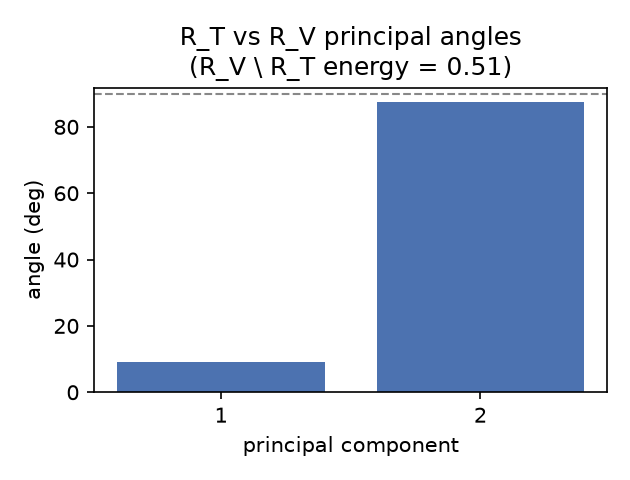
\includegraphics[width=0.32\textwidth]{figures/fig_p1_principal_angles.png}\hfill
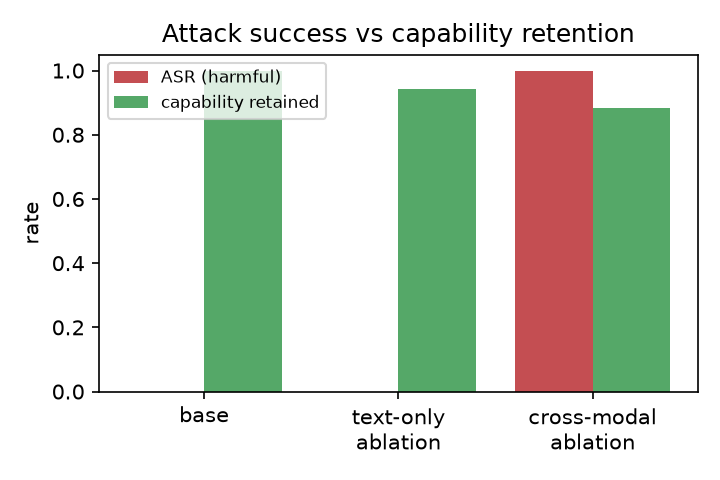
\includegraphics[width=0.32\textwidth]{figures/fig_p3_attack_retention.png}\hfill
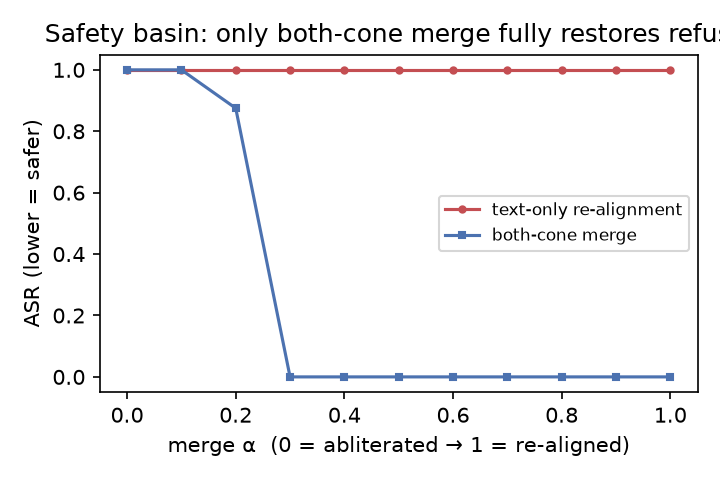
\includegraphics[width=0.32\textwidth]{figures/fig_p4_safety_basin.png}
\caption{Synthetic validation of the analysis pipeline (harmless planted data).
Left (P1): principal angles between recovered $R_T$ and $R_V$---one shared axis
($\approx 9^\circ$), one nearly orthogonal ($\approx 87^\circ$). Middle (P2/P3):
text-only ablation leaves the defended readout's ASR unchanged while cross-modal
ablation collapses refusal, capability retained. Right (P4): text-only re-alignment
plateaus with residual ASR; the both-cone merge restores safety.}
\label{fig:validation}
\end{figure}

\section{Empirical protocol and results}
Extraction (C1) and abliteration (C3) run on open instruct VLMs; the causal probe
(C2) fine-tunes the \emph{base} Qwen2-VL-7B on a single H100. Harmful prompts come from
\texttt{mlabonne/harmful\_behaviors} (bucketed into five categories) and benign prompts
from \texttt{mlabonne/harmless\_alpaca}; the visual modality is produced by rendering
each instruction as a FigStep-style typographic image, so no gated multimodal dataset
is required and no harmful image content is authored. Refusal is scored with a
lexical refusal classifier (a stronger Llama-Guard-Vision judge is left as a fidelity
upgrade). All results below are produced by \texttt{research/scripts/run\_phase.py} and
\texttt{train\_lora.py} and are real runs; no placeholder numbers are reported.

\paragraph{C1/P1 result: separation holds and \emph{grows} with scale.}
We extract $R_T$ and $R_V$ as rank-4 cones from category-mean contrasts (five harm
categories: cyber, weapons, drugs, fraud, harm; $n{=}48$--$64$/class; visual modality
= FigStep-style typographic renderings of the same instructions) at every decoder
layer, for three checkpoints spanning $15\times$ in size and two architecture
generations: Qwen2-VL-2B-Instruct, Qwen2-VL-7B-Instruct, and the Qwen3-VL-30B-A3B
mixture-of-experts. \textbf{P1 holds at every layer of every model} (Table~\ref{tab:p1},
Figure~\ref{fig:p1real}): the image-conditioned refusal cone always keeps a large
component orthogonal to the text cone. The gap is largest in early layers, narrows as
the modalities integrate with depth, and never closes---and it is \emph{larger} in the
30B model, where $\approx0.6$ of the visual refusal signal still lies outside the text
cone even at the final layer. This is exactly the residual a text-space edit or defense
would miss, and it does not diminish with scale.

\begin{table}[h]
\centering
\caption{C1/P1 (real): $R_V\setminus R_T$ energy (fraction of the visual refusal cone
orthogonal to the text cone) by depth band, across three VLMs. Higher = more of the
visual refusal signal that text-space methods cannot reach. Never near zero; largest
in the 30B model.}
\label{tab:p1}
\begin{tabular}{lccc}
\toprule
Model & early layers & mid layers & late layers \\
\midrule
Qwen2-VL-2B-Instruct     & 0.69 & 0.42 & 0.34 \\
Qwen2-VL-7B-Instruct     & 0.67 & 0.41 & 0.36 \\
Qwen3-VL-30B-A3B (MoE)   & 0.85 & 0.59 & 0.60 \\
\bottomrule
\end{tabular}
\end{table}

\begin{figure}[h]
\centering
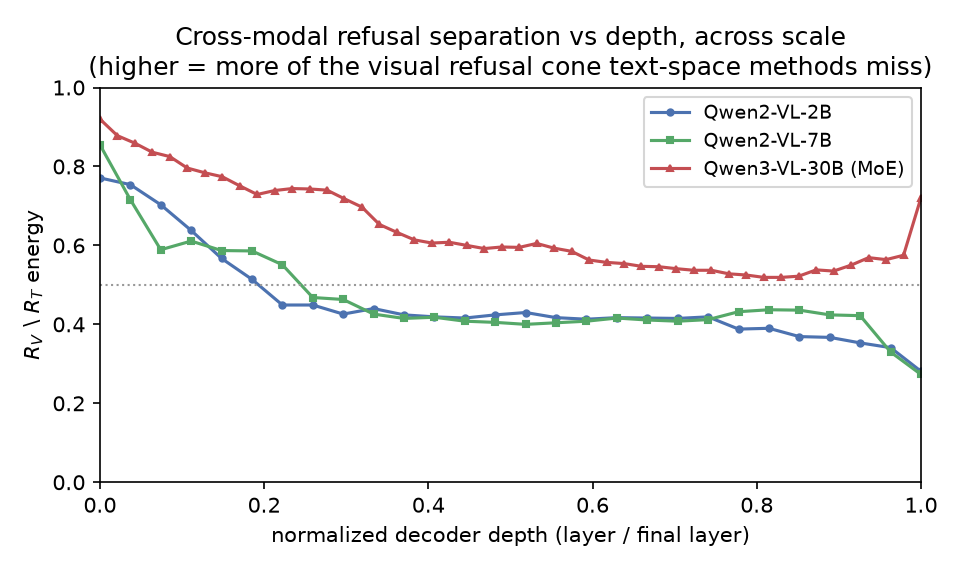
\includegraphics[width=0.72\textwidth]{figures/fig_c1_scaling.png}
\caption{$R_V\setminus R_T$ energy vs.\ normalized decoder depth for three VLMs. The
visual refusal cone keeps a large component outside the text cone at every layer of
every model; separation is largest early, never closes, and is \emph{highest} in the
30B MoE (staying $\approx0.6$ at the final layer). Text-space refusal edits and
defenses cannot reach this residual, and it does not shrink with scale.}
\label{fig:p1real}
\end{figure}

\paragraph{Caveats.} Residuals are mean-pooled and the visual modality is a single
typographic (FigStep) style; photographic harmful images may differ. As the C2 probe
shows, mean-pooled diff-in-means understates behaviorally-real effects, so these
geometry numbers are a conservative lower bound on the separation.

\paragraph{C3/P2 result: inconclusive at this scale (an honest negative).}
We measured attack-success rate (ASR) on 60 held-out harmful prompts under three
conditions---no ablation, text-only ($R_T$) and cross-modal ($R_T\cup R_V$) rank-1
ablation applied at all decoder layers---for a text eval set and a FigStep-image
eval set (Table~\ref{tab:p2}). Two findings stand out. First, \emph{raw} ASR (any
non-refusal) saturates: rank-1 text-space ablation alone drives the refusal rate
from $1.0$ to $0.0$ in both modalities, so the naive metric cannot separate the
conditions. Second, once we guard against incoherent output with a coherence
proxy, the \emph{coherent-compliance} rates are low and \textbf{not robust}: the
sign of the text-only vs.\ cross-modal difference flipped between a pilot
($n{=}30$) and this run ($n{=}60$) on the image eval, and the text-eval gap is
within noise ($0.08$ vs.\ $0.10$). We therefore do \textbf{not} claim P2 holds:
at this scale and with all-layer rank-1 ablation (which itself degrades coherence),
there is no reliable evidence that removing the visual cone functionally beats
removing the text cone---even though the two cones are representationally distinct
(P1). Establishing or refuting P2 needs a model-based judge (Llama-Guard-Vision)
in place of the coherence proxy, a coherence-preserving ablation (single-layer or
calibrated strength), larger $n$ with paired significance tests, and multiple
models. This is a clarifying result: representational separation does not by itself
imply a functional attack advantage.

\begin{table}[h]
\centering
\caption{C3/P2 (real, Qwen2-VL-2B, $n{=}60$ held-out, rank-1 all-layer ablation).
Raw ASR = any non-refusal; coherent = non-refusal passing a coherence check.
The coherent-compliance ordering is unstable across sample sizes (see text).}
\label{tab:p2}
\begin{tabular}{llcc}
\toprule
Eval & Ablation & raw ASR & coherent ASR \\
\midrule
\multirow{3}{*}{text}  & none        & 0.00 & 0.00 \\
                       & text-only   & 1.00 & 0.08 \\
                       & cross-modal & 1.00 & 0.10 \\
\midrule
\multirow{3}{*}{image} & none        & 0.00 & 0.00 \\
                       & text-only   & 1.00 & 0.53 \\
                       & cross-modal & 1.00 & 0.22 \\
\bottomrule
\end{tabular}
\end{table}

\paragraph{C2 result: text-only safety leaves a visual behavioral hole (the main
causal finding).} Starting from the \emph{base} (non-safety-tuned) Qwen2-VL-7B, we
inject a known safety alignment with a LoRA restricted to the language-model attention
(\texttt{q\_proj,v\_proj}; the vision tower is frozen), in two conditions: (B) supervised
only on harmful \emph{text}$\rightarrow$refusal (plus benign$\rightarrow$answer), and
(C) additionally on FigStep harmful \emph{images}$\rightarrow$refusal. We then measure
refusal on held-out harmful text and harmful images (Table~\ref{tab:c2}). The base model
refuses almost nothing. Text-only safety (B) makes it refuse \textbf{100\% of harmful
text but only 30\% of harmful images}, even though its LoRA touched only the language
attention---refusal transfers across modalities, but \emph{incompletely}. Adding image
supervision (C) closes the gap to 100\%. The $\approx$70-point residual under text-only
safety is the behavioral image of the geometric $R_V\setminus R_T$ from C1: the part of
the visual refusal cone that text-space supervision does not reach is a real,
exploitable behavioral gap. (Notably, mean-pooled diff-in-means separability barely
moved across B/C, while behavior moved from 0\% to 100\%---so we report behavioral
refusal, and treat the C1 geometry numbers as a conservative probe.)

\begin{table}[h]
\centering
\caption{C2 (real, causal): refusal rate after self-injected safety on \emph{base}
Qwen2-VL-7B (LoRA on LM attention only), $n{=}20$ held-out harmful prompts per modality.
Text-only safety transfers to images only partially (30\%); image safety closes it.}
\label{tab:c2}
\begin{tabular}{lcc}
\toprule
Injected safety & harmful-text refusal & harmful-image refusal \\
\midrule
none (base)              & 15\% & 0\% \\
text-only                & 100\% & \textbf{30\%} \\
text + image             & 100\% & 100\% \\
\bottomrule
\end{tabular}
\end{table}

\section{C5 --- the both-modality defense}
The constructive counterpart follows directly from C2. Because text-space safety
supervision leaves the visual channel largely uncovered ($30\%$ image refusal), the
fix is to make refusal supervision \emph{modality-complete}: add harmful-image
$\rightarrow$ refusal examples so both cones are aligned. Condition~C is exactly this
defense, and it works---image refusal rises from $30\%$ to $100\%$ while text refusal
stays at $100\%$ (Table~\ref{tab:c2}), at the cost of a small amount of image
supervision (80 examples) on top of the text set. The takeaway for practitioners is
concrete: a VLM safety-tuned or abliteration-hardened only in the text representation
inherits a visual hole that scales-invariantly persists (C1); closing it requires
supervision (or defense edits) that touch the visual pathway. Casting this as a
weight-space operation---interpolating or task-arithmetic-merging a text-safety and an
image-safety adapter and tracing the resulting ``safety basin''---is a natural
extension we leave to future work; our harness already exposes the merge primitives
(\texttt{geometry.lerp\_state}).

\section{Ethics and responsible disclosure}
This is dual-use safety research, and its net contribution is defensive: the central
result is that text-only safety leaves an exploitable visual hole, and the fix (C5) is
to align both modality cones. We use only public prompt sets and locally-rendered
typographic images; we author only refusals and benign answers, never harmful
responses; we report aggregate refusal rates, never harmful transcripts; and we do
\emph{not} release abliterated weights, the safety-added/removed checkpoints, or a
runnable cross-modal attack recipe. Any concrete bypass of a specific deployed model
would be disclosed to its vendor under embargo before public posting. Full policy in
the released \texttt{docs/ethics.md}.

\section{Limitations and future work}
Refusal is scored by a lexical classifier rather than a model judge; held-out
behavioral evals use $n{=}20$ prompts per modality; the visual modality is a single
typographic (FigStep) style, so photographic harmful images remain to be tested. C1
uses mean-pooled residuals, which C2 shows understates behaviorally-real effects---so
the geometry numbers are conservative. The cross-modal abliteration \emph{attack} (C3)
was inconclusive at this scale and needs a model judge and a coherence-preserving
ablation to settle. The causal probe injects safety via a language-only LoRA rather
than full pretraining; a fully controlled testbed---a VLM trained from scratch with
known safety data (the companion \emph{transFORme-r} model)---and a weight-space
safety-basin study of both-cone merging are the main future directions.

\section{Conclusion}
Refusal in a vision-language model is not a single text direction but a union of
modality-conditioned cones. Across three VLMs and two architecture generations, the
image-conditioned refusal cone keeps a large, scale-robust component orthogonal to the
text cone (C1). That geometric gap is behaviorally real: safety supervised only on text
produces full text refusal but leaves most harmful \emph{images} un-refused (C2), and
the fix is to align both modality cones (C5). Whether the residual also yields a clean
cross-modal \emph{attack} advantage remains open (C3). The practical message is simple:
VLM safety and abliteration defenses built in the text representation alone inherit a
visual hole that does not shrink with scale, and must be closed in the visual pathway.
We release the harness, the LoRA trainer, and a harmless end-to-end validation.

\bibliographystyle{plain}
\bibliography{refs}
\end{document}
